\subsection{Número promedio de viajes}

Los datos abiertos de MiBici contienen un identificador de usuario, por lo que se puede saber el número de viajes realizados en un día por todos los usuarios. En base a este tiempo calculado en minutos, se usaron las ecuaciones \ref{eq:monthly_hourly_mean}, \ref{eq:monthly_hourly_var}, \ref{eq:daily_hourly_mean} y \ref{eq:daily_hourly_var}. Los resultados obtenidos son los siguientes:

\subsubsection{Promedio y desviación estandar mensual por hora}

En la figura \ref{fig:monthly_hourly_count_travel} se visualiza que existe un aumento en el número de viajes entre los meses septiembre y diciembre. Lo cual coincide con lo antes planteado con las figuras \ref{fig:monthly_hourly_distance} y \ref{fig:monthly_hourly_time}. En la figura \ref{fig:monthly_hourly_var_count_travel} se observa como el número de usuarios tiene una variación mayor a las 8, y 18 horas. Esto puede deberse a la elección de los usuarios por que servicio de transporte público les hes mejor tomar en un día.

\begin{figure}[H]
    \centering
    \begin{subfigure}[b]{8cm}
        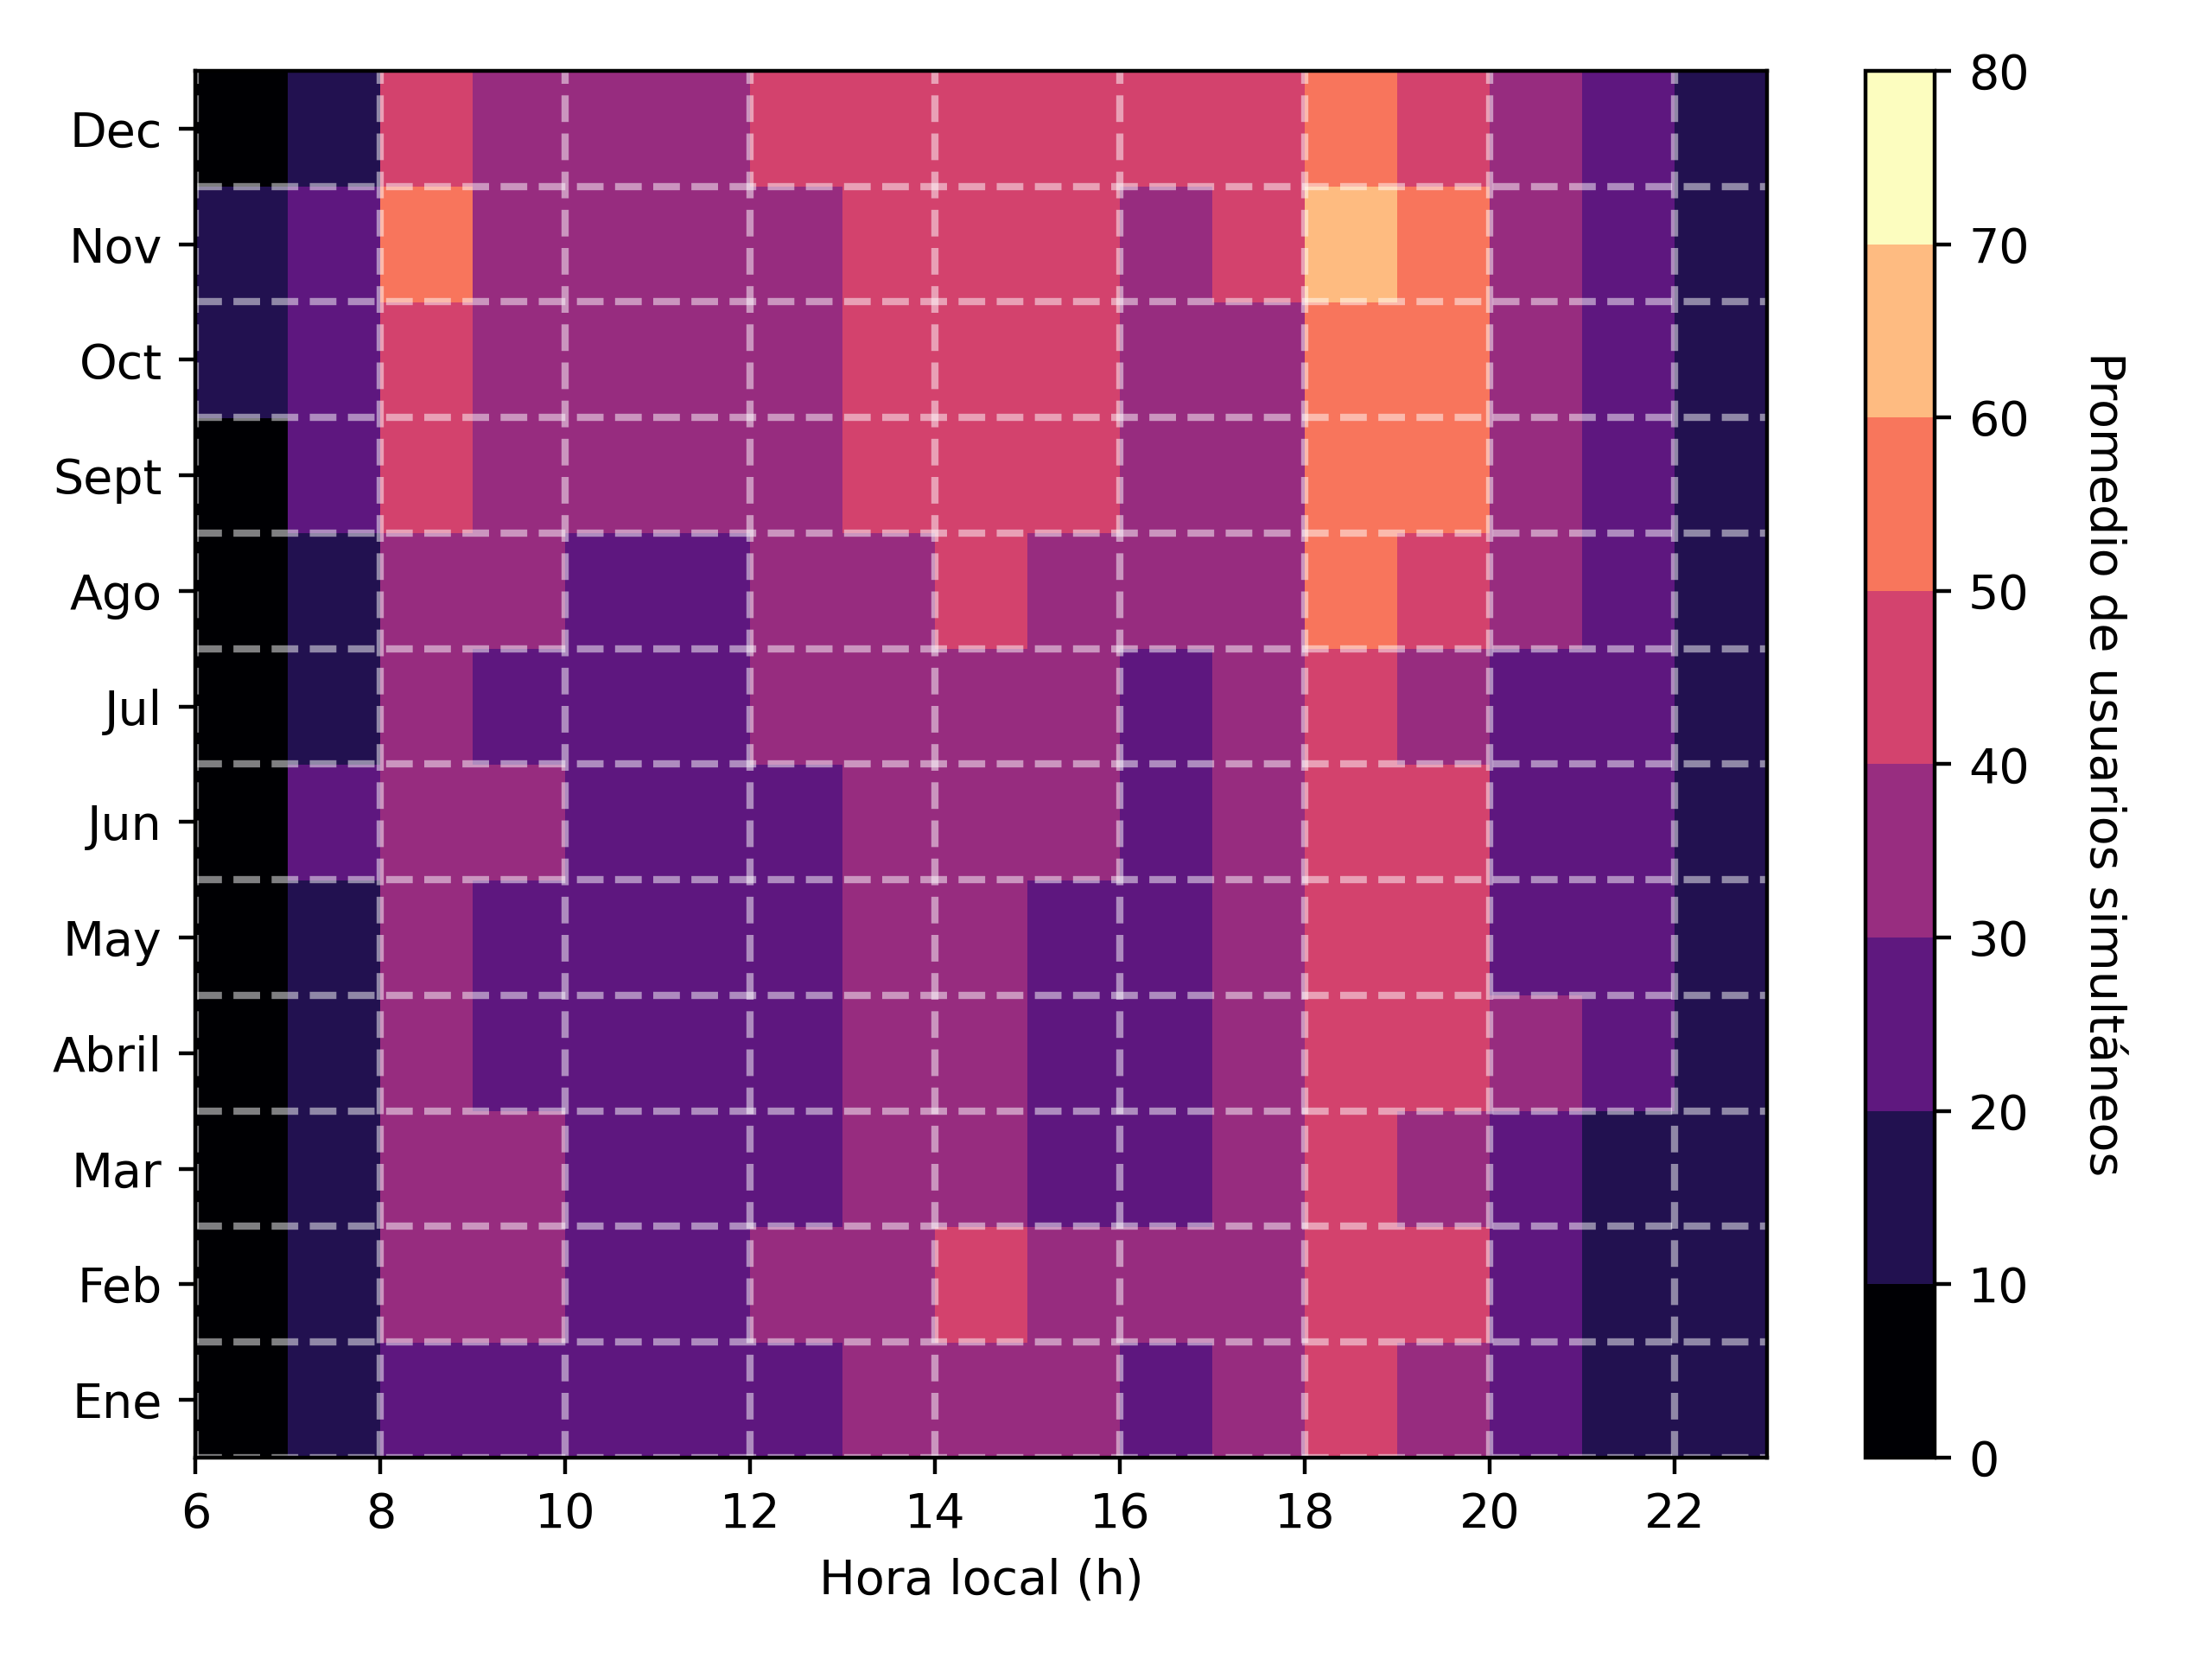
\includegraphics[width=8cm]{Graphics/monthly_hourly_mean_count_travel.png}
        \caption{Promedio mensual del número de usuarios.}
        \label{fig:monthly_hourly_mean_count_travel}
    \end{subfigure}
    \begin{subfigure}[b]{8cm}
        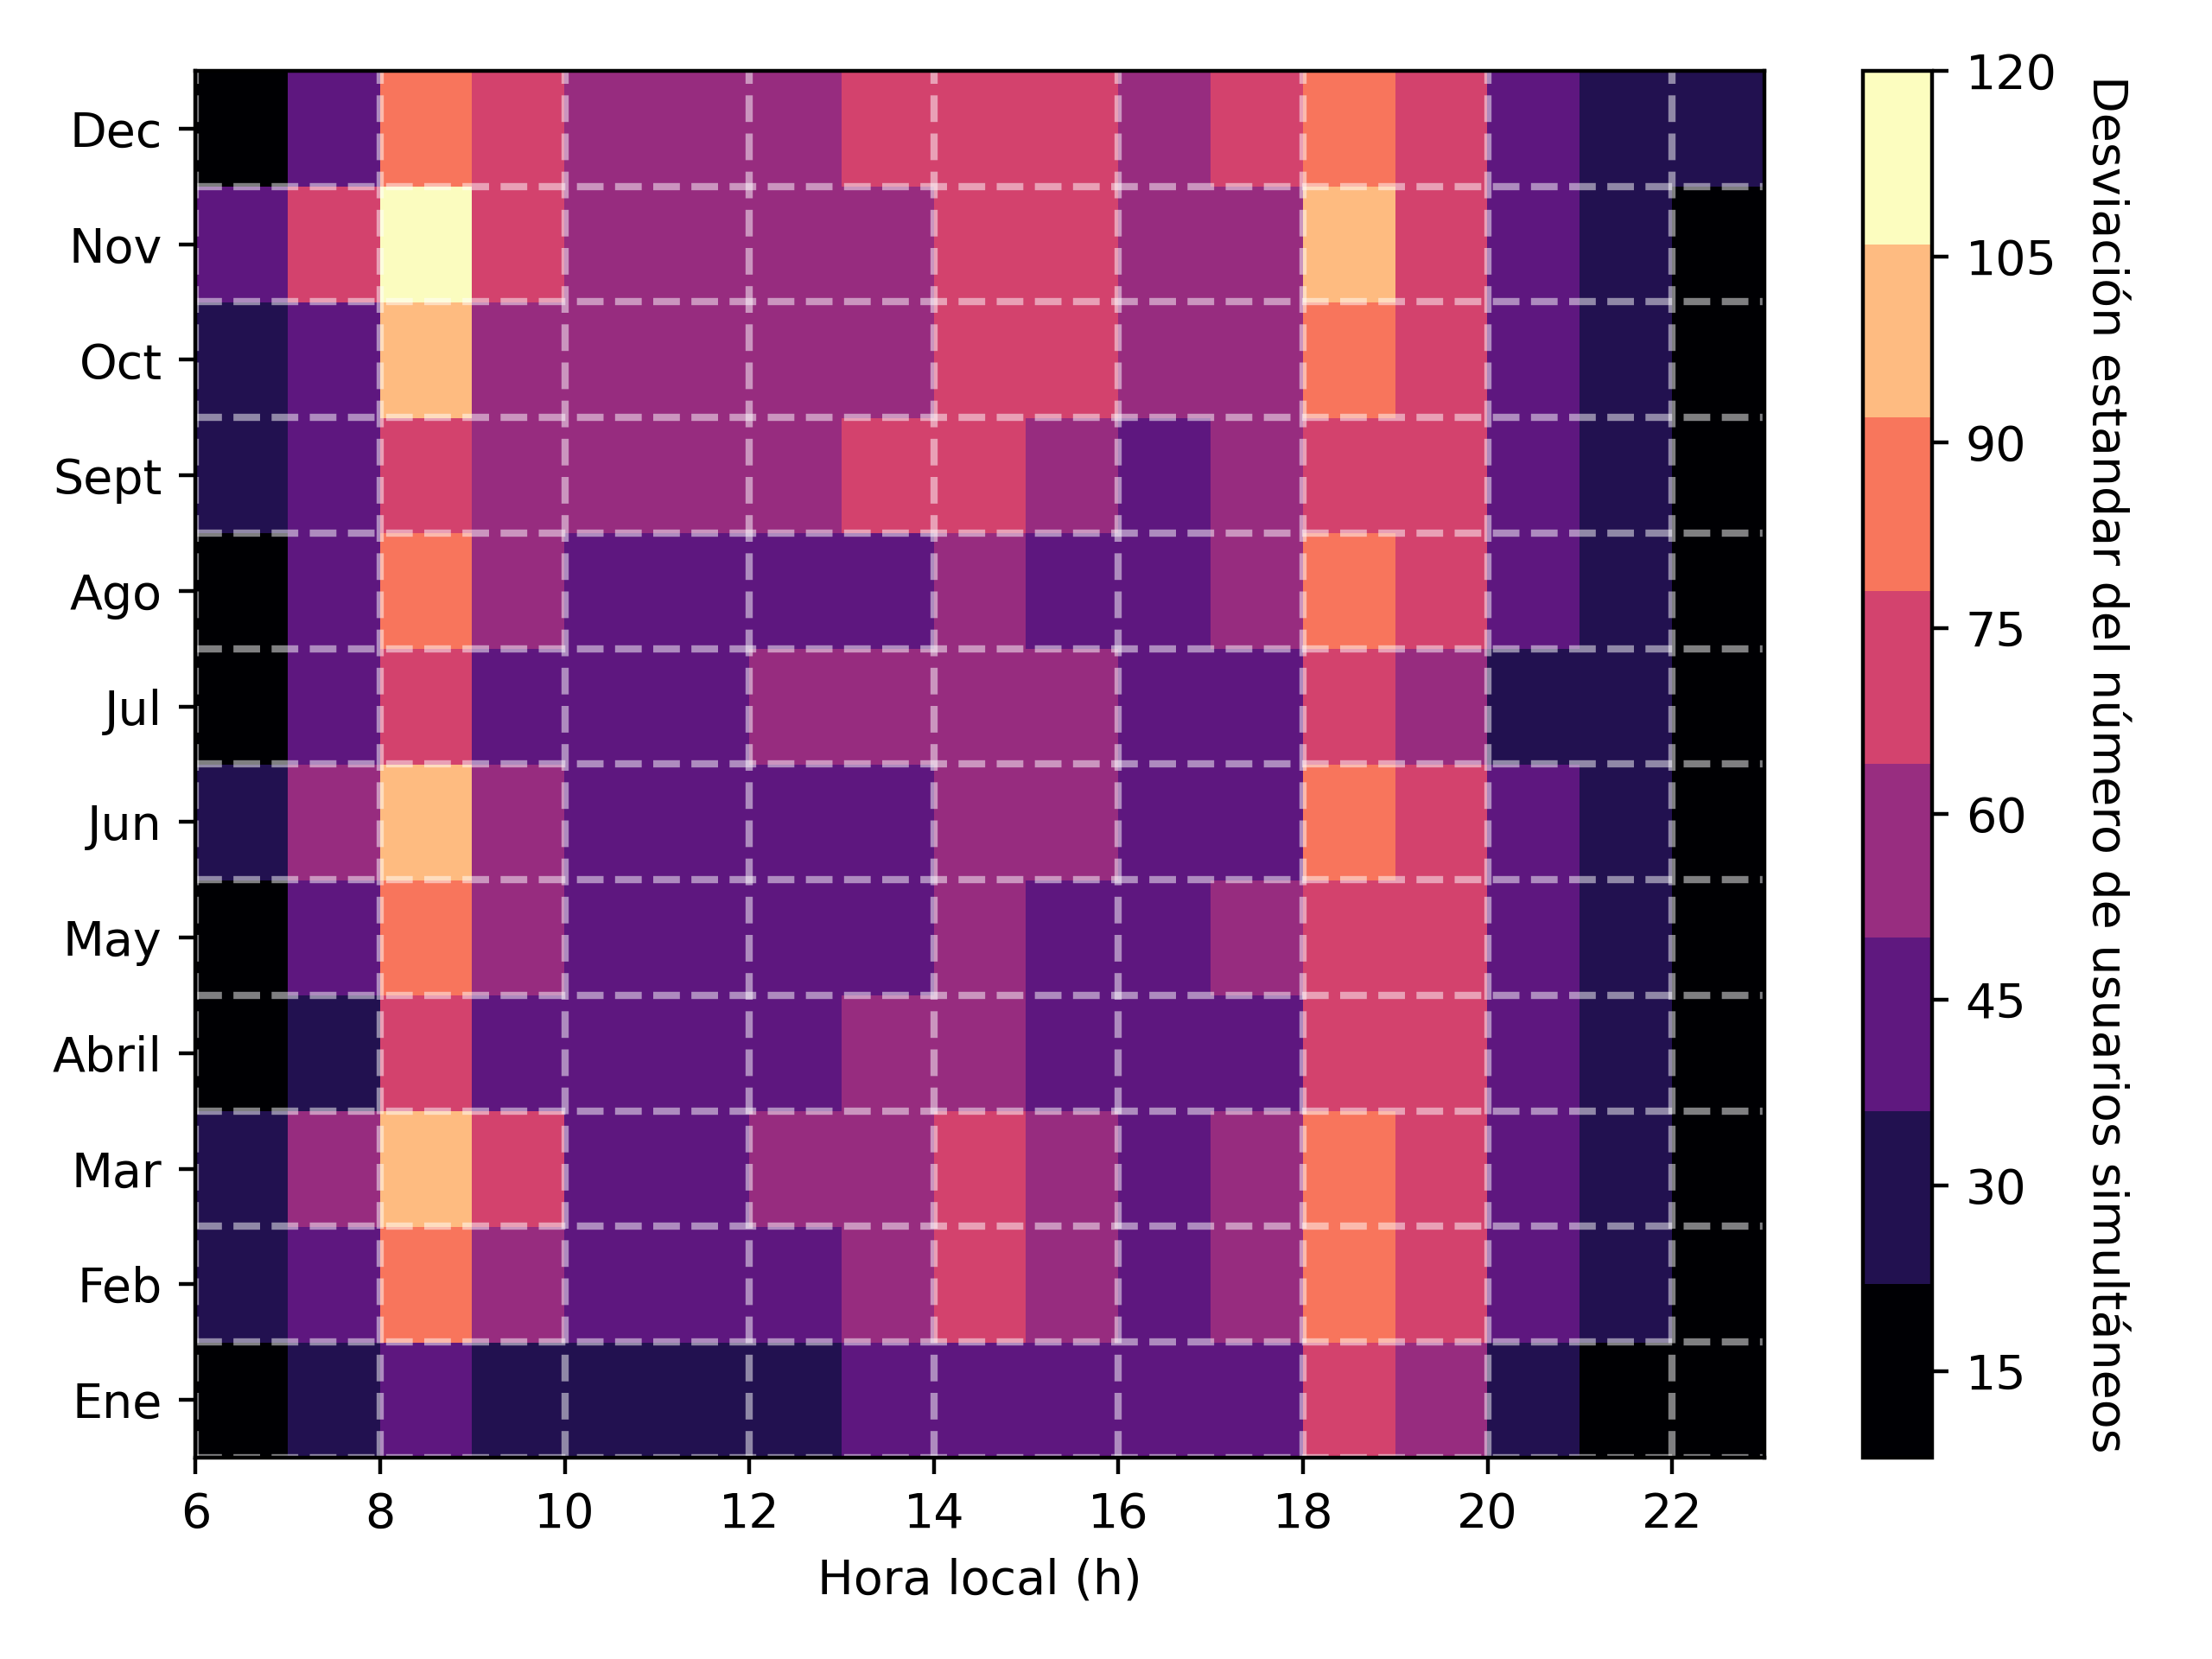
\includegraphics[width=8cm]{Graphics/monthly_hourly_var_count_travel.png}
        \caption{Desviación estandar del número de usuarios.}
        \label{fig:monthly_hourly_var_count_travel}
    \end{subfigure}
    \caption{Tiempo de uso promedio y desviación estandar mensual por hora de lo usuarios calculadas con las ecuaciones \ref{eq:monthly_hourly_mean} y \ref{eq:monthly_hourly_var}.}
    \label{fig:monthly_hourly_count_travel}
\end{figure}

\subsubsection{Promedios diarios semanales por hora}

En la figura \ref{fig:daily_hourly_mean_count_travel} se aprecia que existe una predilección en utilizar el servicio de bicicleta entre semana a las 8 y 16 horas. Existiendo un mínimo en el horario de 17 a 23 horas los días sabados y domingos. Con la figura \ref{fig:daily_hourly_var_count_travel} se observa que en el periodo donde existe un máximo, este presenta una gran variación, lo cual concuerda con lo encontrado en la figura \ref{fig:monthly_hourly_var_count_travel}. Por ende, se puede suponer que los usuarios que utilizan el servicio en ese periodo de tiempo pueden no ser recurrentes y usarlo cuando les sea necesario, más no es su primera opción.

\begin{figure}[H]
    \centering
    \begin{subfigure}[b]{8cm}
        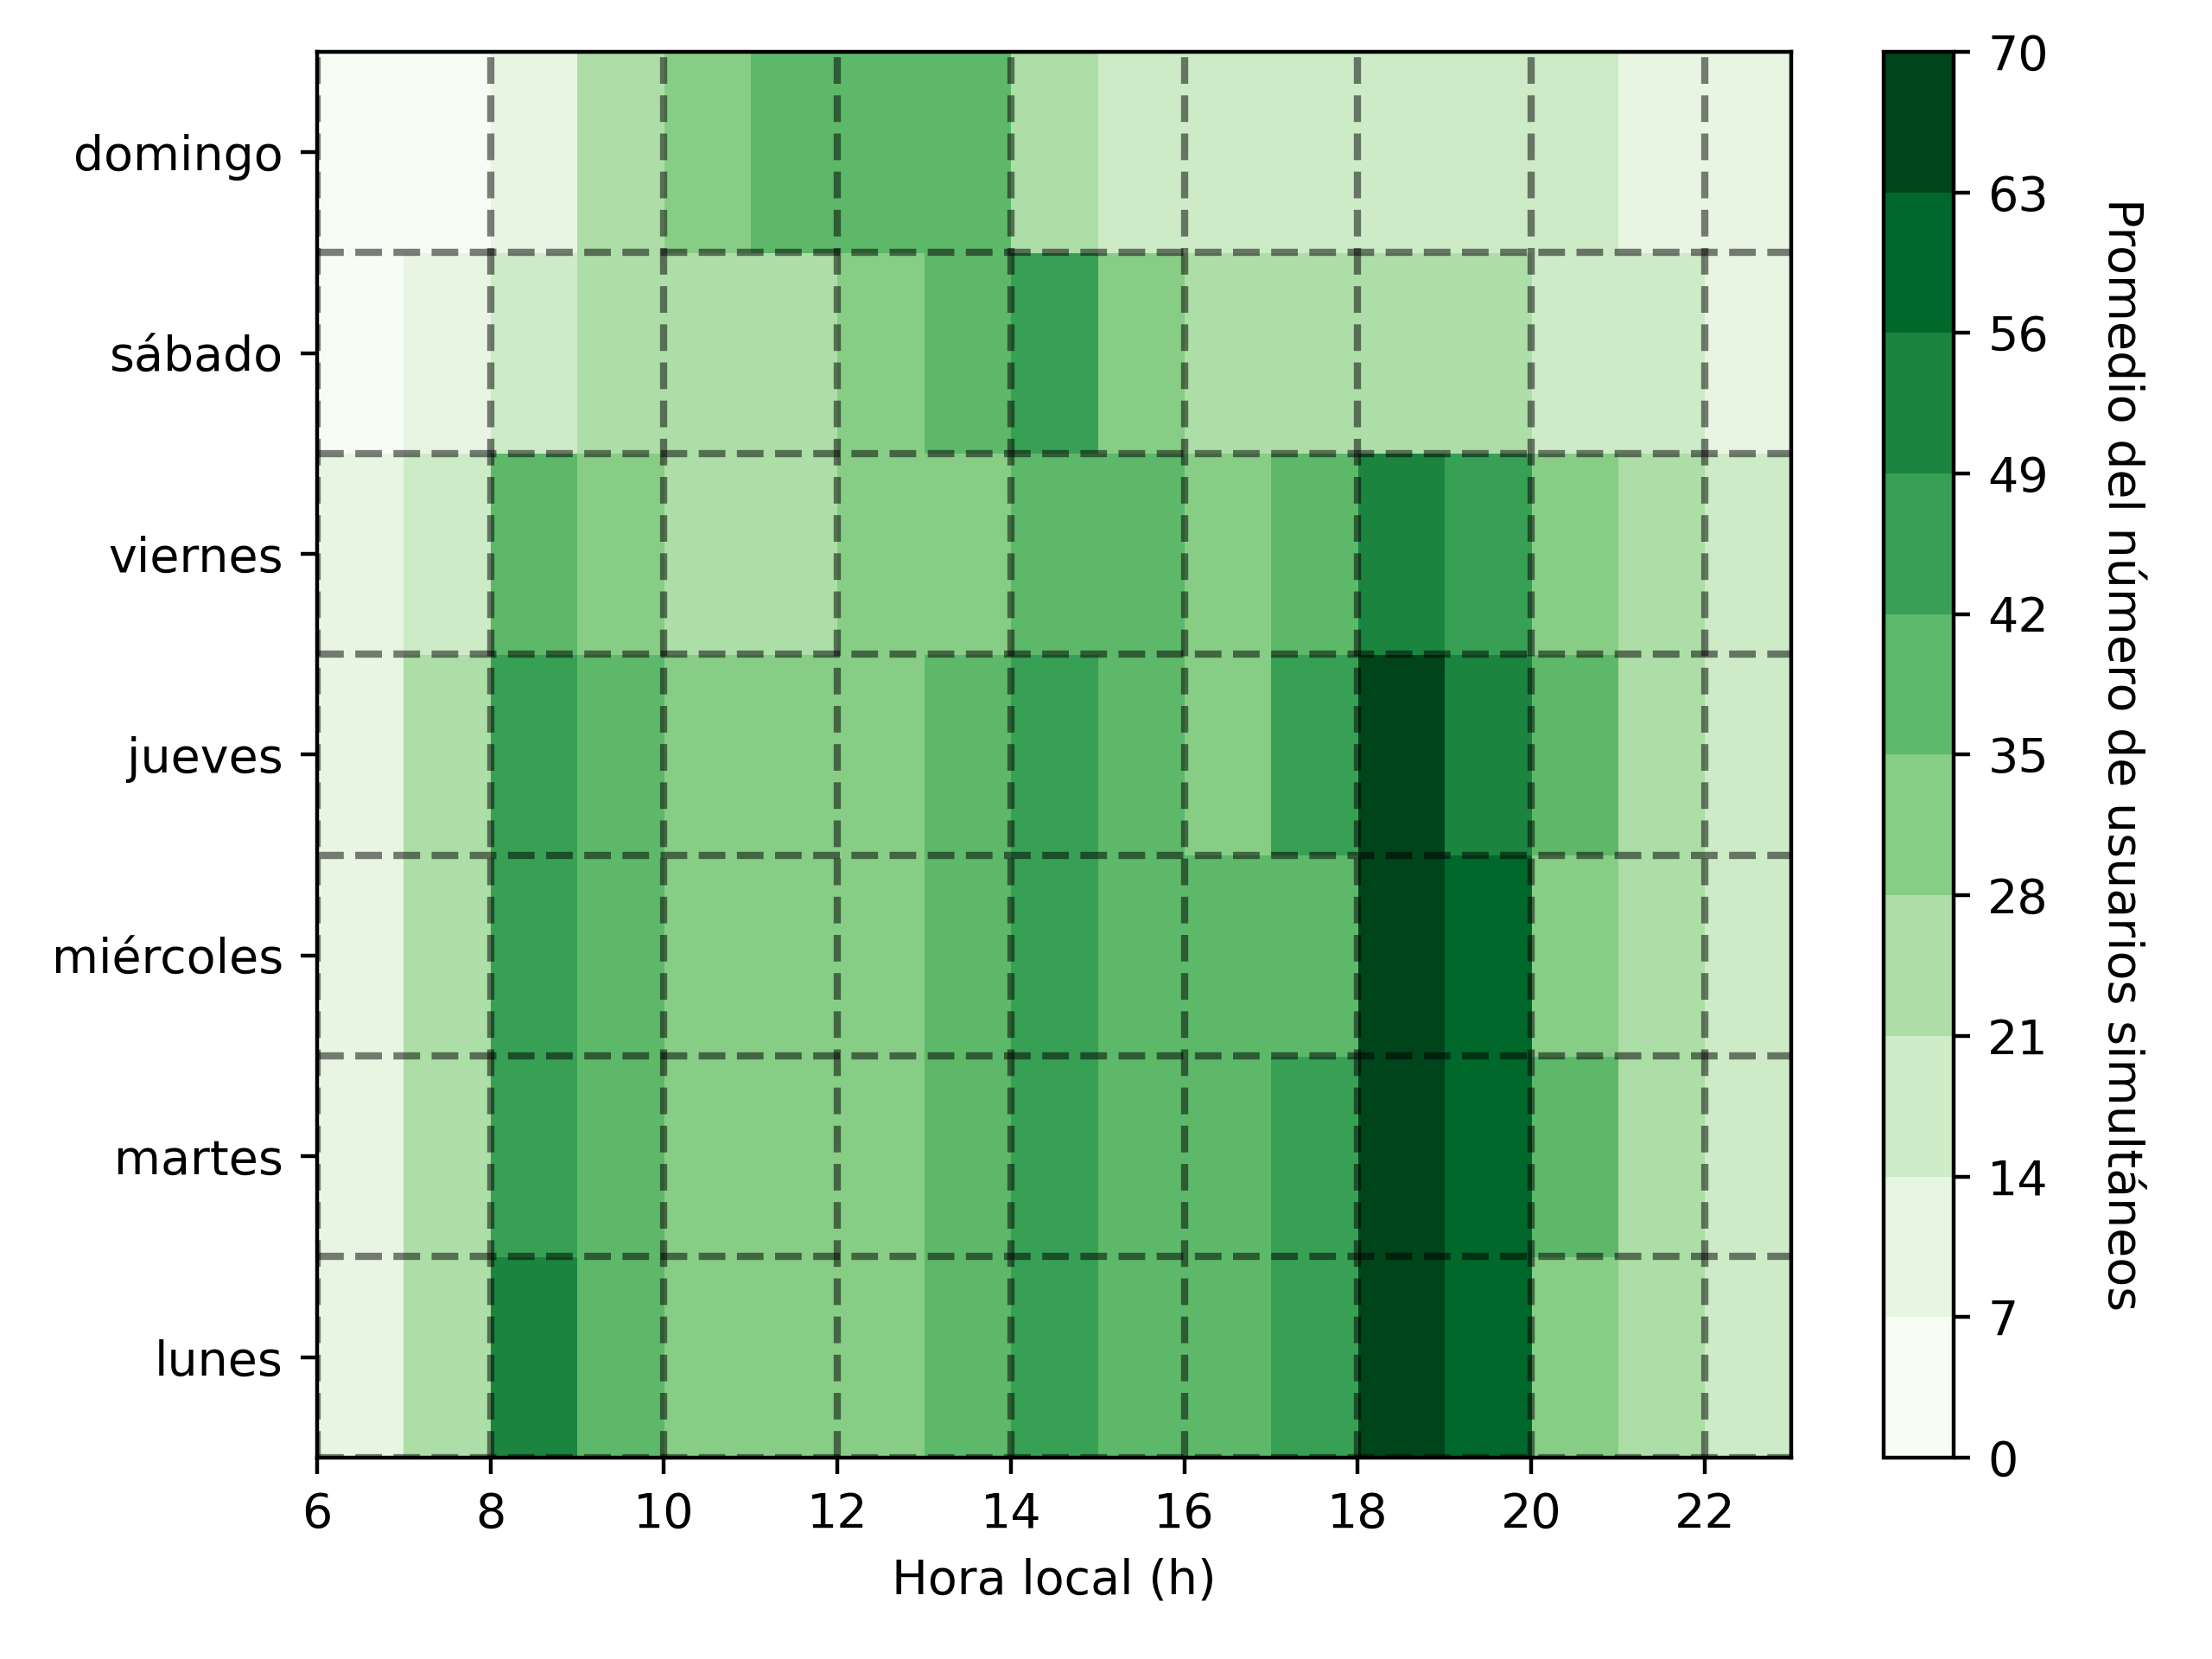
\includegraphics[width=8cm]{Graphics/daily_hourly_mean_count_travel.png}
        \caption{Promedio diaria del número de usuarios semanal.}
        \label{fig:daily_hourly_mean_count_travel}
    \end{subfigure}
    \begin{subfigure}[b]{8cm}
        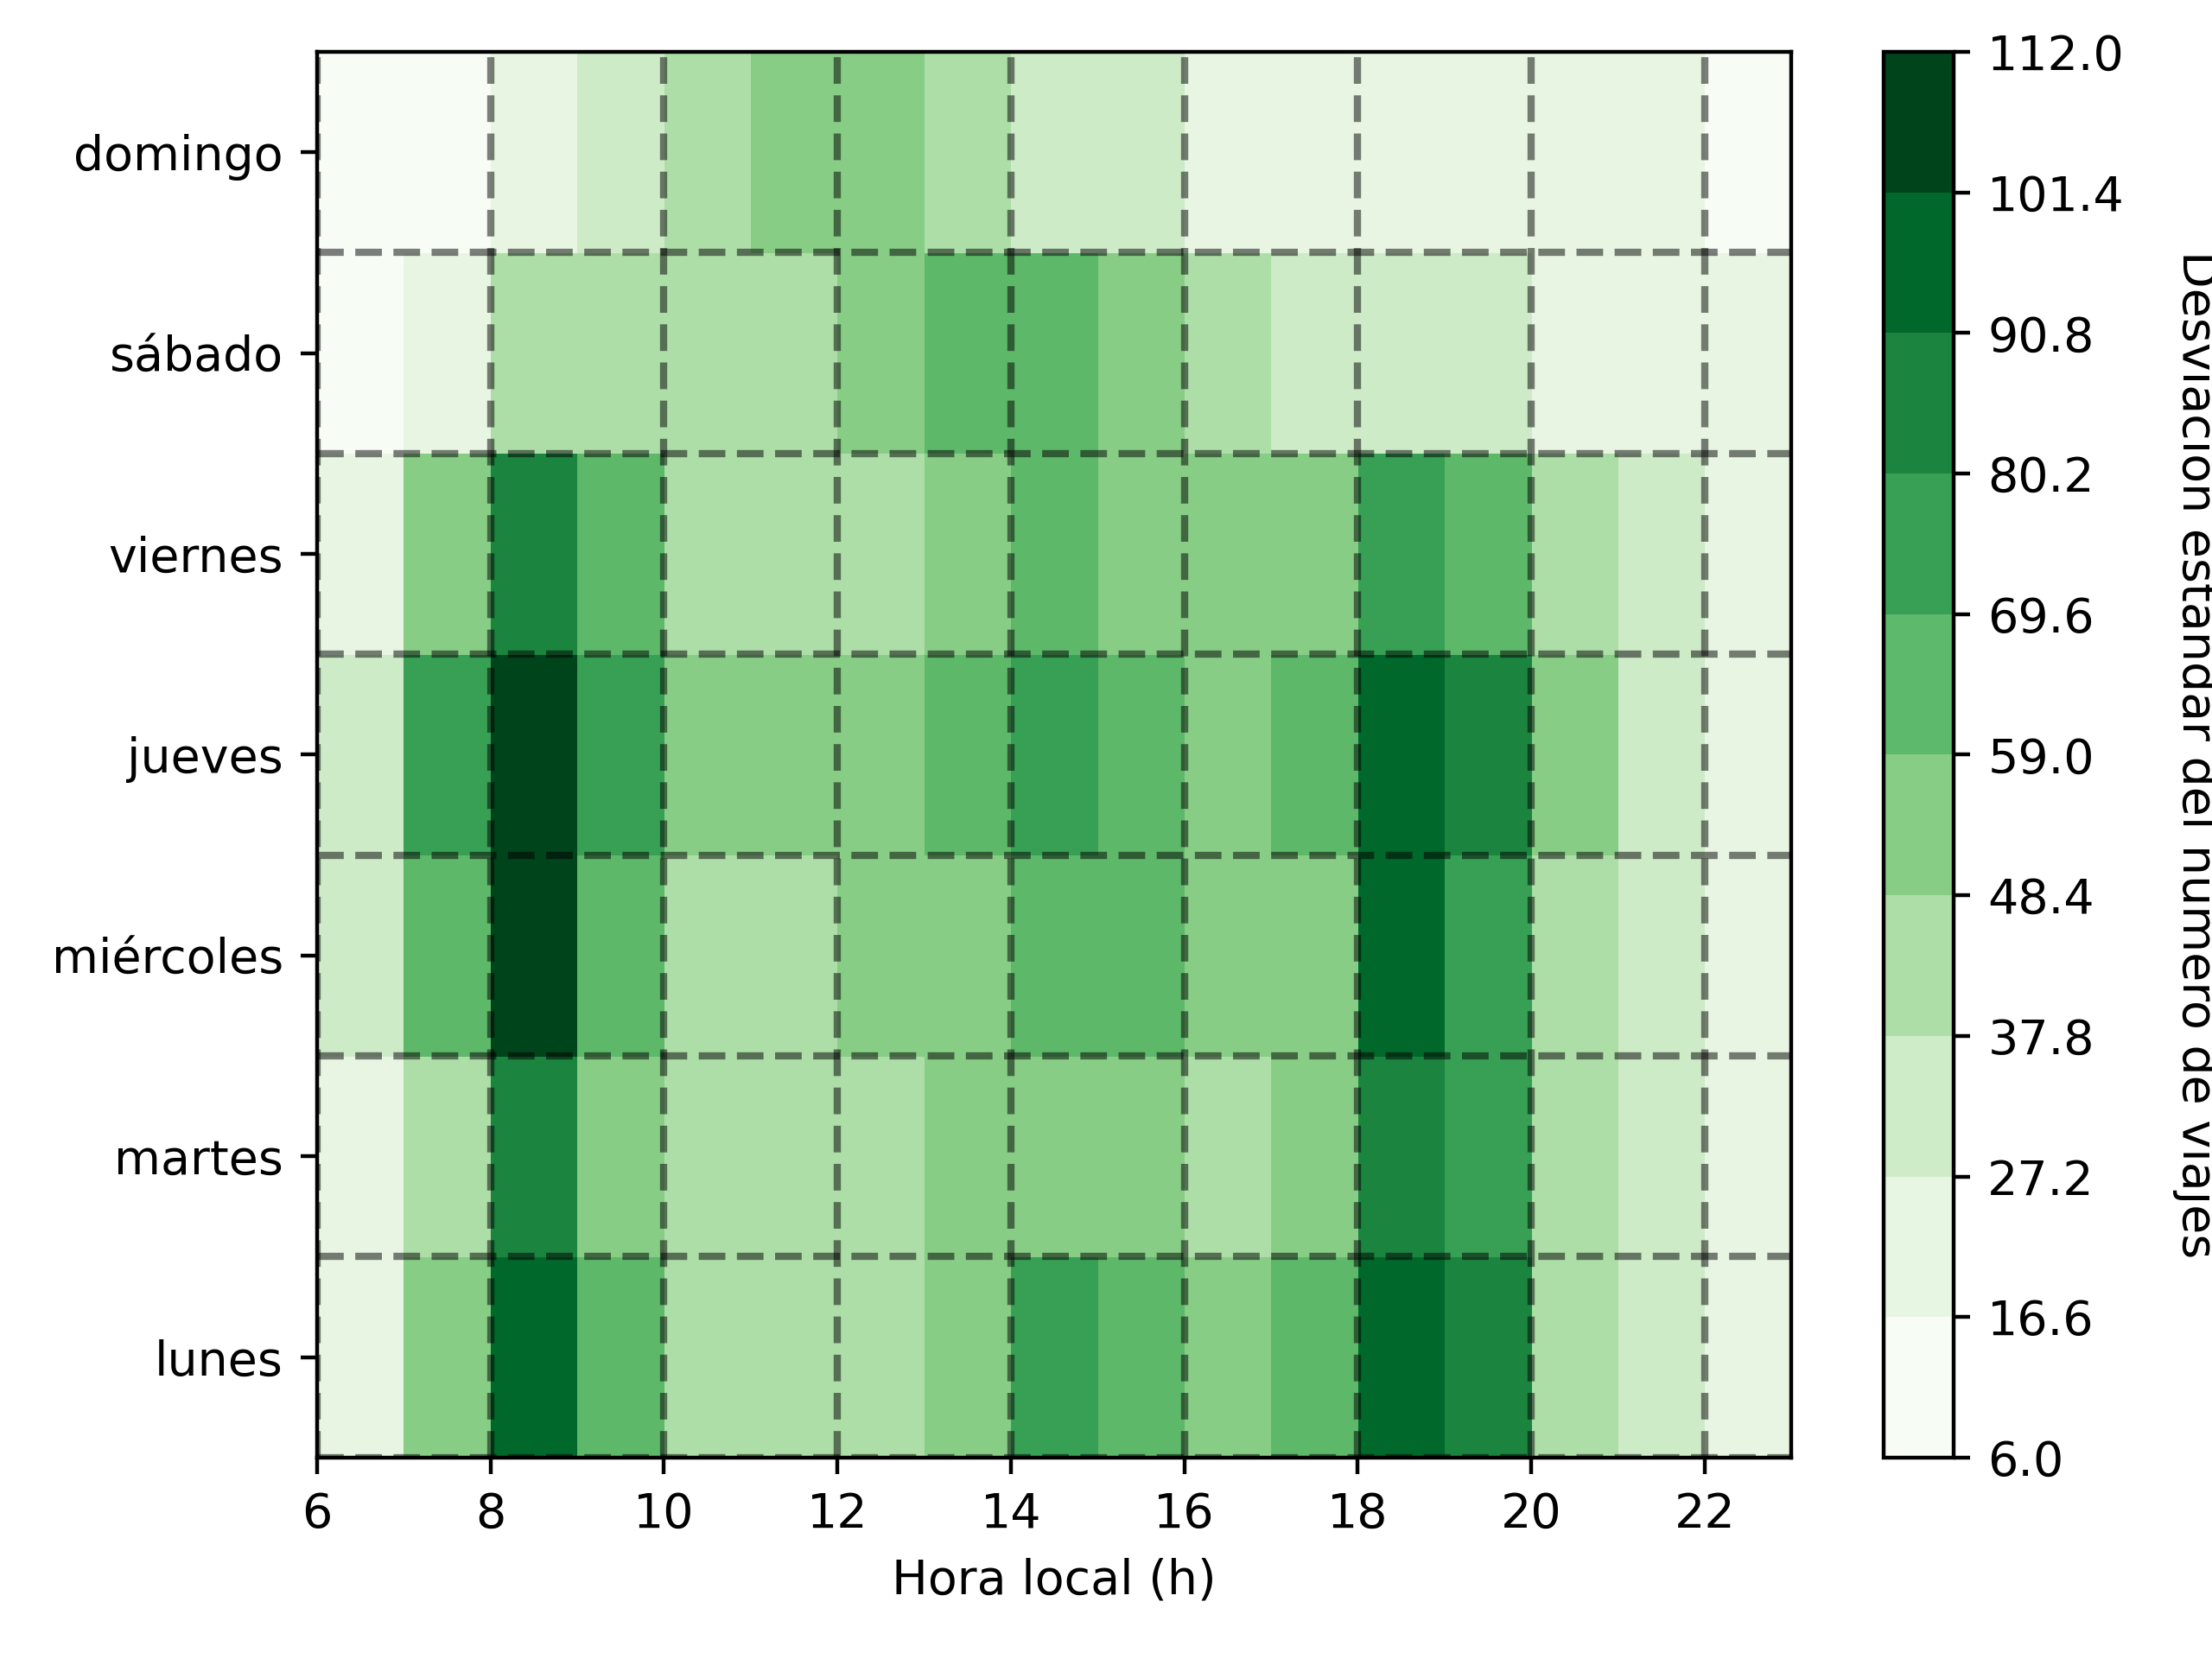
\includegraphics[width=8cm]{Graphics/daily_hourly_var_count_travel.png}
        \caption{Desviación estandar del número de usuarios semanal.}
        \label{fig:daily_hourly_var_count_travel}
    \end{subfigure}
    \caption{Número de usuarios promedio y desviación estandar diaria semanal por hora calculados con las ecuaciones \ref{eq:daily_hourly_mean} y \ref{eq:daily_hourly_var}.}
    \label{fig:daily_hourly_count_travel}
\end{figure}